%%%%%%%%%%%%%%%%%%%%%%%%%%%%%%%%%%%55%%
\begin{frame} [plain]
    \frametitle{}
    \Background[1] 
    \begin{center}
    { {\huge 第一章:绪论 }}
    \end{center}  
    \addtocounter{framenumber}{-1}   
\end{frame}
%%%%%%%%%%%%%%%%%%%%%%%%%%%%%%%%%%
\section{课程简介}

\begin{frame}[t]
    \frametitle{课程目标}
        \begin{enumerate}
            \Item Learn the formal theory of Quantum Mechanics
            \IItem How physical systems are described in Quantum Mechanics.
            \Item How to solve problems in Quantum Mechanics.
        \end{enumerate}
\end{frame}
\begin{frame} [t]
    \frametitle{分数构成}
        \begin{enumerate}
            \Item Normal results 20\%
            \Item Midterm examination results 20\%
            \Item Final examination results 60\%
        \end{enumerate}
\end{frame}

\begin{frame} [t]
    \frametitle{教学效果}
    \centering
    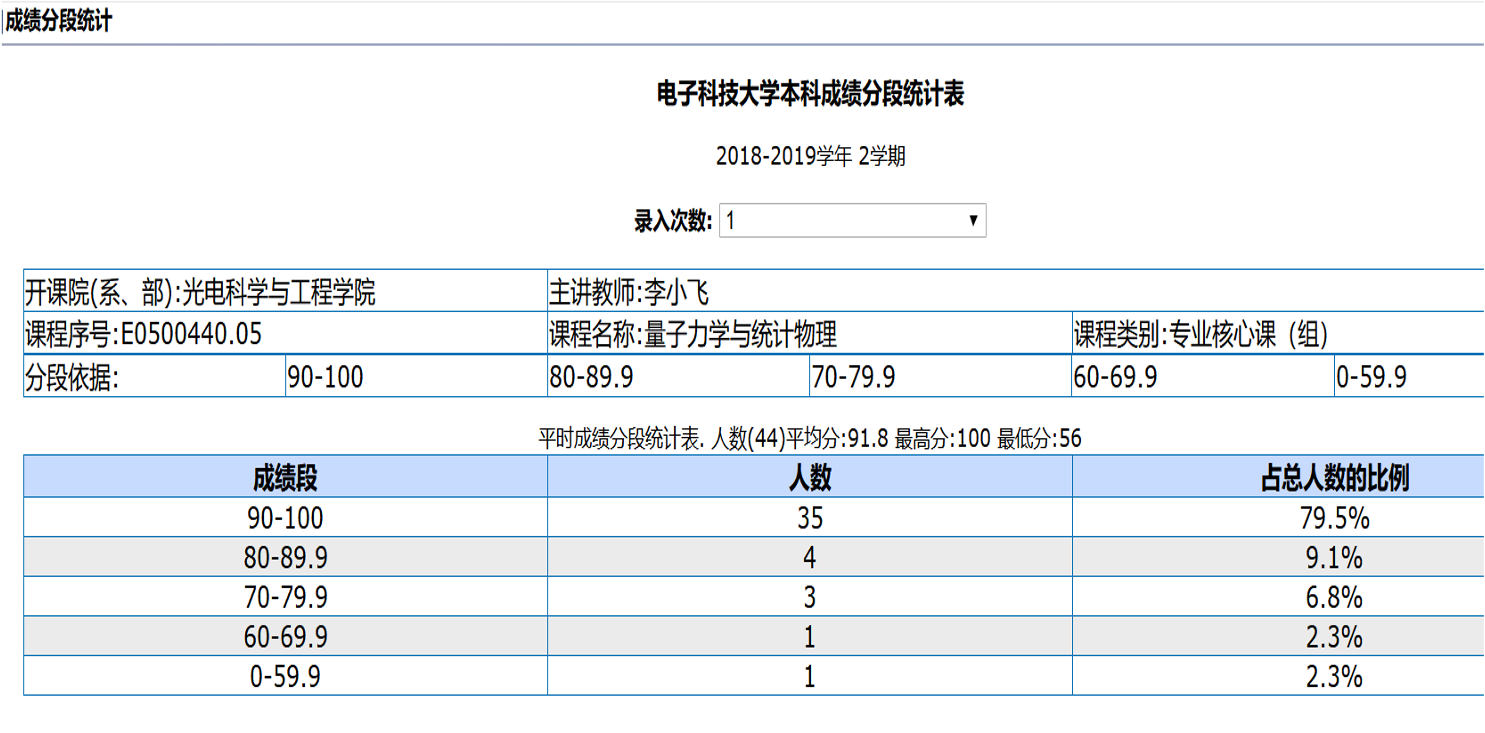
\includegraphics[width=1.0\textwidth,height=5.0cm]{figs/exam1.png}
\end{frame}

\begin{frame}[t]
    \frametitle{参考书目}
        \begin{itemize}
            \Item 《量子力学》卷I,II, 曾谨言, 科学出版社, 2008           
            \Item Principles of quantum mechanics, shankar
            \Item Modern quantum mechanics, shankar
            \Item Lectures on quantum mechanics, weinberg
            \Item Principles of quantum mechanics, Dirac
        \end{itemize}
\end{frame}

\begin{frame}[t]
    \begin{tcolorbox4}[三条军规]    
        \begin{enumerate}
            \Item Objects are wave-particles and can be in states of superposition
            \Item Rule 1 holds as long as you don't measure
            \Item Measurement gives random results
        \end{enumerate}
    \end{tcolorbox4} 
\end{frame}

\section{能量子假说}

\subsection{伟大成就}

\begin{frame}[t]
    \frametitle{经典物理伟大成就}
    \begin{tcolorbox3}
    [Great successes in Classical Physics]
        \begin{enumerate}
            \Item Newtonian mechanics
            \Item Maxwell's electromagnetism
            \Item Thermodynamic laws
        \end{enumerate}
    \end{tcolorbox3}  
    \begin{quotation}
        "There is nothing new to be discovered in physics now. All that remains is 
        more and more precise measurements"   \\
        \rightline{$\cdots$ Lord Kelvin (1900)\hspace{3em}}
    \end{quotation}
\end{frame}

\begin{frame}
    \frametitle{}
    \begin{quotation}
        "But the beauty and clearness ... is obscured by two small puzzling clouds \faCloud "  \\
        \rightline{$\cdots$ Lord Kelvin (1900.4)\hspace{3em}}   
    \end{quotation}
    ~~ \vspace{0.3em}
    \begin{tcolorbox4}[两朵乌云]    
        \begin{enumerate}
        \Item Michelson-Morley experiment
        \Item Black body radiation
        \end{enumerate}
    \end{tcolorbox4} 
\end{frame}

\begin{frame}
    \frametitle{迈克尔逊-莫雷实验}
    \begin{center}
    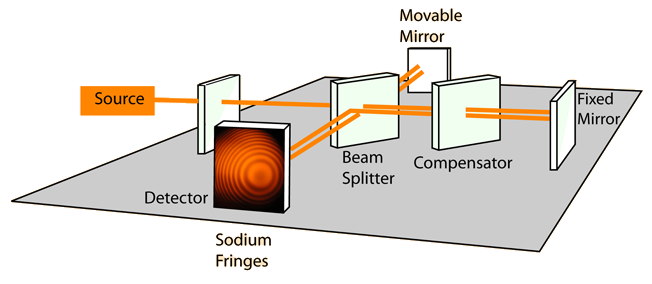
\includegraphics[width=0.8\textwidth]{figs/michel.png}
    \end{center}
There is no displacement of the interference bands. \dots 
the Stationary Ether is thus shown to be incorrect
\end{frame}

\begin{frame}
    The theory of relativity is established 
    \begin{center}
        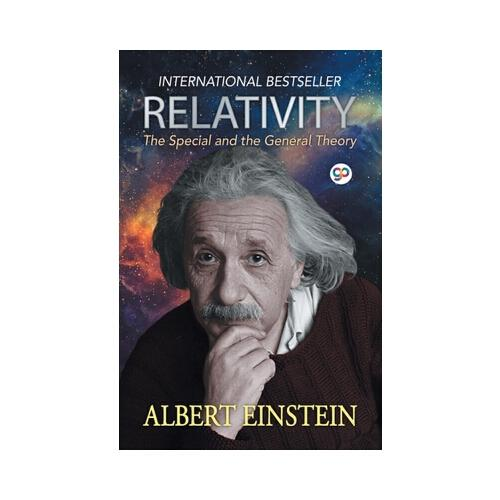
\includegraphics[width=0.4\textwidth]{figs/relativity.jpg}
    \end{center}   
    Greatly changed our view of time and space. Mainly useful in two aspects: high-speed motion, and strong gravitational field. 
\end{frame}

\begin{frame}
    \frametitle{黑体辐射实验}
    \begin{center}
    \includegraphics[width=0.7\textwidth]{figs/2021-12-01-23-47-27.png}
    \end{center}
    No mathematical function to describe the curves exactly 
\end{frame}
\begin{frame}
    Quantum mechanics is established  
    \begin{center}
        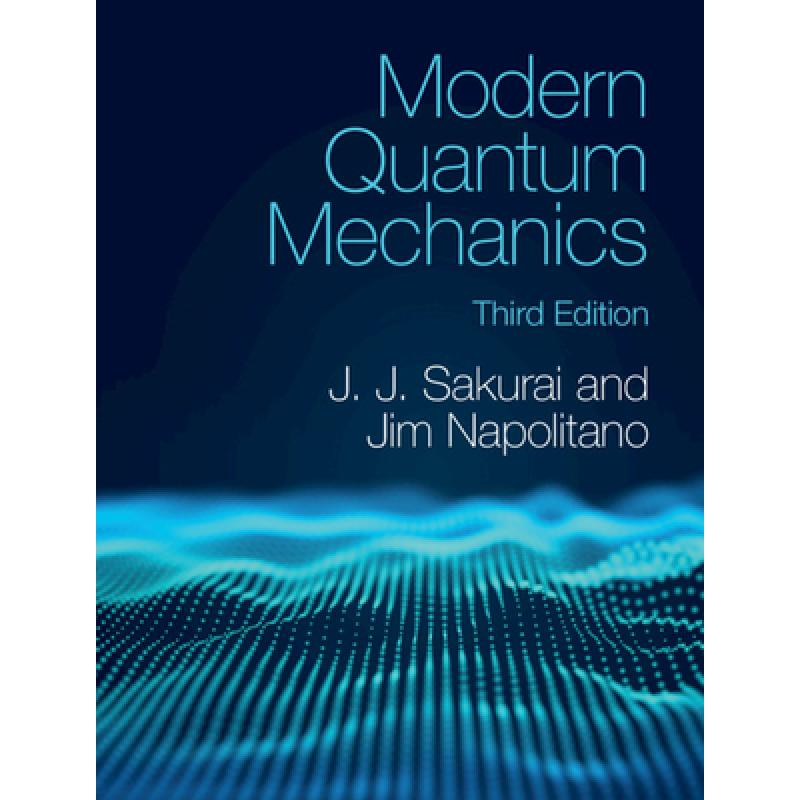
\includegraphics[width=0.45\textwidth]{figs/mqm.jpg}
    \end{center}   
    It is a theory about matter.
\end{frame}

\begin{frame}
    \frametitle{现代科学基石}
    \begin{center}
        \includegraphics[width=0.75\textwidth]{figs/stone.png}
    \end{center}   
\end{frame}

%%%%%%%%%%%%%%%%%%%%%%%%%%%%%%%%%%%%
\subsection{普朗克公式}
%%%%%%%%%%%%%%%%%%%%%%%%%%%%%%%%%%%%

\begin{frame}
    \frametitle{Black body radiation}
    \begin{tcolorbox1}{Definition}
    Black body:  absorb all electromagnetic waves in any temperature
    \end{tcolorbox1}
    \begin{center}
        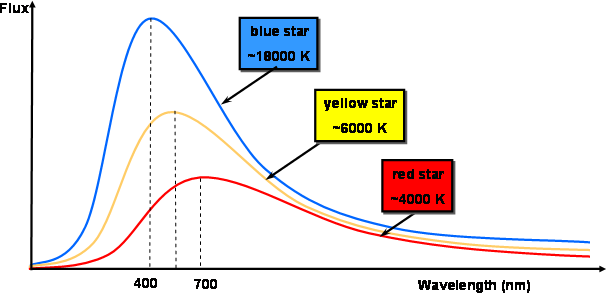
\includegraphics[width=0.6\textwidth]{figs/blackbody_radn_curves.png}
    \end{center}
    \textbf{\color{deepred} Most interestingly}, what is the mathematical function that describes all of these curves?
\end{frame}

\begin{frame}
    \frametitle{三个经验公式}
    \begin{center}
        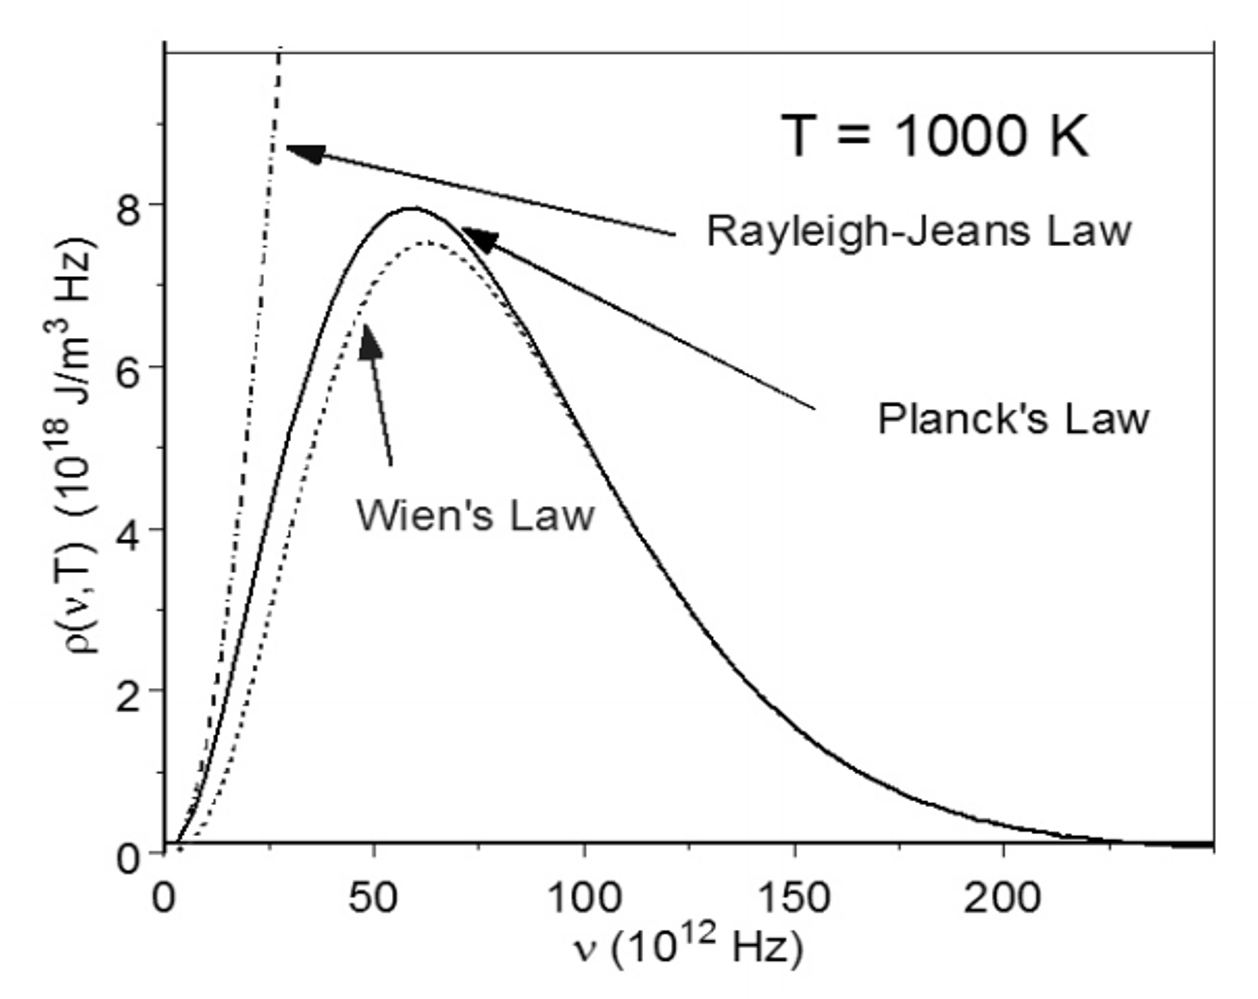
\includegraphics[width=0.7\textwidth]{figs/threelaws.png}
    \end{center}
\end{frame}

\begin{frame} [t]
    \frametitle{维恩公式}
    \begin{equation*}
        \rho(\nu) d \nu=c_{1} \nu^{3} e^{-c_{2} \nu / T} d \nu 
    \end{equation*}
    Derived from electromagnetism (1893), but described well only in high frequency region.\\ 
    {\color{deepred} Nobel Prize in physics(1911)}\\
\end{frame}

\begin{frame}[t]
    \frametitle{瑞-金公式}
    \begin{equation*}
        \rho(\nu, T) d \nu=\frac{8 \pi}{c^{3}} \nu^{2} k T d \nu 
    \end{equation*}
    Derived from thermodynamics (1900), but described well only in low frequency region.\\ 
   {\color{deepred} Nobel Prize in physics(1904)}\\ \vspace{0.3em}
   {\color{deepblue} \bullet Ultraviolet Catastrophe:} 
    \begin{equation*}
         \int_0 ^\infty \frac{8 \pi}{c^{3}} \nu^{2} k T d \nu \to \infty 
    \end{equation*}
\end{frame}

\begin{frame}
    \frametitle{普朗克公式}
    On 1900-10-19, at the German Physical Society, 
    Max Planck presented a resolution to {\color{deepblue} Ultraviolet Catastrophe} 
    \begin{equation}
        \boxed{\rho(\nu, T) d \nu=\frac{8 \pi}{c^{3}} \frac{h \nu^{3}}{e^{h \nu / K T}-1} d \nu}
    \end{equation}
    Obtained from experimental data via interpolation technique, described well in whole region \\
    {\color{deepred} Nobel Prize in physics(1918)}\\
\end{frame}

\begin{frame}[t]
    \begin{tcolorbox1}{Problems}
        How to derive the formula from existing theory.
    \end{tcolorbox1}
    \begin{tcolorbox2}{Solution}
        On 1900-12-14, Planck gives out his solution based on the Energy Quantum Hypothesis  
    \end{tcolorbox2}
\end{frame}

%%%%%%%%%%%%%%%%%%%%%%%%%%%%%%%%%%%%
\subsection{能量子假说}
%%%%%%%%%%%%%%%%%%%%%%%%%%%%%%%%%%%%
\begin{frame}
    \begin{tcolorbox4}[Energy quantum hypothesis]
    Assuming the oscillators of the cavity could only radiate at a discrete amounts of energy
    \begin{equation}
        E=n\varepsilon
    \end{equation}
    where, the $\varepsilon$ is the unit of the energy (quanta) determined by the oscillator' frequency 
    \begin{equation}
        \varepsilon=h\nu
    \end{equation}
    and the $h=6.6260693(11)\times10^{-34} J\cdot s $ is the Planck constant. 
    \end{tcolorbox4}
\end{frame}

\begin{frame}
    Based on Boltzmann distribution law,
    \begin{equation*}
        \frac{N_{i}}{N}=\frac{\exp \left(-\frac{E_{i}}{k T}\right)}{\sum_{i} \exp \left(\frac{-E_{i}}{k T}\right)}
    \end{equation*}
    \bullet when the energy is continuous,the distribution between $E - dE$ should be 
    \begin{equation*}
        \frac{e^{-E / k T}}{\int\limits_{0}^{\infty} e^{-E / k T} d E}
    \end{equation*}  
    the average energy 
    \begin{equation*}
        <E>=\int\limits_{0}^{\infty} E \frac{e^{-E / k T}}{\int\limits_{0}^{\infty} e^{-E / k T} d E} d E
    \end{equation*}
\end{frame}

\begin{frame}
    \begin{equation*}
        \begin{split}
            <E> &= -kT \frac{Ee^{-E / k T}\vert_0 ^\infty-\int\limits_{0}^{\infty} e^{-E / k T} d E } {\int\limits_{0}^{\infty} e^{-E / k T} d E }\\  
                &= kT
        \end{split}  
    \end{equation*} 
    \bullet when the energy is discrete,the distribution should be   
    \begin{equation*}
        \frac{e^{-E / k T}}{\int\limits_{0}^{\infty} e^{-E / k T} d E} 
        \to \frac{e^{-E / k T}}{\sum\limits_{0}^{\infty} e^{-E / k T}} 
        \to \frac{e^{-nh\nu / k T}}{\sum\limits_{0}^{\infty} e^{-nhv / k T}} 
    \end{equation*}    
\end{frame}

\begin{frame}
    the average energy 
    \begin{equation*}
        \begin{split}
            <E> &= \sum\limits_{0}^{\infty} nh\nu\frac{e^{-nh\nu / k T}}{\sum\limits_{0}^{\infty} e^{-nh\nu / k T}} \\
            &= -h\nu \frac{d}{dx} \frac{n e^{-nx}}{\sum\limits_{0}^{\infty} e^{-nx}} \\
            &= \frac{h\nu}{e^{h\nu/kT}-1} 
        \end{split} 
    \end{equation*}
    We get
    \begin{equation*}
        \text{(continuous)} \quad k T \rightarrow \frac{h \nu}{e^{ h \nu / k T}-1} \quad \text{(discrete)} 
    \end{equation*}
\end{frame}

\begin{frame}
    In Rayleigh-Jeans formula
    \begin{equation*}
        \rho(\nu, T) d \nu=\frac{8 \pi}{c^{3}} \nu^{2} k T d \nu 
    \end{equation*}
    the item $kT$ should be replaced by $\dfrac{h \nu}{e^{ h \nu / k T}-1}$
    \begin{equation*}
        \rho(\nu, T) d \nu=\frac{8 \pi}{c^{3}} \frac{h \nu^{3}}{e^{h \nu / K T}-1} d \nu
    \end{equation*}
    It is the Planck's formula exactly 
\end{frame}

\begin{frame}
    \begin{tcolorbox4}[Revolutionary Significance]
        Planck's Energy Quantum Hypothesis broke through the constraints of classical physics and 
        opened the door of quantum mechanics 
    \end{tcolorbox4}
\end{frame}

\begin{frame}
    \frametitle{}
    \tcbbtitle{一只会下金蛋的鹅}
    \centering
    \tcbb[0.68]
    {
    历史上,普朗克,德拜,艾伦菲斯特,劳厄,洛伦兹,庞加莱,泡利,玻色,爱因斯坦等从多角度推导过普朗克公式,每一次推导都给物理学带来了新的知识内容 
    }

 《黑体辐射公式的多种推导及其在近代物理构建中的意义》- 返朴|曹则贤
\end{frame}

%\begin{frame}
%    \begin{tcolorbox}[colback=yellow!10,colframe=red!75!black,title=THE END]
%    In 1927, Dirac got the Planck's formula from Quantum Mechanism.  
%    \end{tcolorbox}
%\end{frame}

\begin{frame}
    \frametitle{}
    \begin{tcolorbox3}[学术讨论]
        普朗克黑体辐射公式重要,还是能量量子化观念重要?\\
        能量量子化只是一种数学处理工具?
    \end{tcolorbox3}
\end{frame}

%\begin{frame}
%    \frametitle{Homework}
%    \begin{enumerate}
%        \item Planck's Energy Quantum Hypothesis
%        \item What's the quanta
%        \item Deriving the Rayleigh-Jeans formula and Wien's formula from Planck's formula
%    \end{enumerate}
%\end{frame}
%%%%%%%%%%%%%%%%%%%%%%%%%%%%%%%%%%%%%%%%%%%%%%%%%%%%%%%%%%%%%%%%%%%